\section{Processi primari}
\subsection{Fornitura}
\subsubsection{Descrizione}

Il processo di fornitura viene svolto al fine di comprendere al meglio la richiesta di appalto del \glo{proponente}: viene svolta un'analisi approfondita che ne stabilisce criticità e punti di forza, i quali verranno spiegati nello \SdF{}. Per sancire il legame tra \glo{proponente} e fornitore è necessaria la definizione di un contratto, che formalizza le fasi della realizzazione del prodotto finale, tra cui consegna e manutenzione. Per instaurare un rapporto di collaborazione proficuo, il gruppo intende mantenere un dialogo costante col \glo{proponente} in modo da accordarsi sugli aspetti che il prodotto dovrà soddisfare, definendo vincoli e \glo{requisiti} e stimandone costi e tempistiche.
Le fasi che compongono il suddetto processo sono: 
\begin{itemize}
	\item avvio;
	\item approntamento di risposte alle richieste;
	\item contrattazione;
	\item pianificazione;
	\item esecuzione e controllo;
	\item revisione e valutazione;
	\item consegna e completamento.
\end{itemize}
\subsubsection{Scopo e aspettative}

Il documento include le norme a cui i membri del gruppo \Gruppo{} devono fare riferimento al fine di ottenere il ruolo di fornitori del \glo{proponente} \proponente{} e dei committenti \textit{Prof. Tullio Vardanega} e \textit{Prof. Riccardo Cardin}. Ognuno è tenuto ad attenersi a quanto scritto nella suddetta sezione durante tutte le fasi di sviluppo del capitolato \textit{C7}.
Per ottenere un riscontro efficace sul lavoro svolto, il gruppo \gruppo{} si propone di instaurare e mantenere un dialogo continuo e un costante rapporto collaborativo con l'azienda \proponente{}.

\subsubsection{Studio di fattibilità}
L'attività di Studio di fattibilità, che sfocia nell'omonimo documento, serve a trovare le motivazioni per la scelta di un capitolato tra quelli proposti.
Il documento \SdF{} viene redatto dopo un'attenta analisi svolta dai membri.
Per ogni capitolato sono indicate:
\begin{itemize}
	\item \textbf{Informazioni generali}: elenco delle informazioni di base, quali nome del progetto, il \glo{proponente} e il committente;
	\item \textbf{Descrizione e finalità}: sintesi del prodotto, comprendente le caratteristiche principali che vengono richieste e l'obiettivo da raggiungere;
	\item \textbf{Tecnologie interessate}: elenco delle tecnologie richieste per lo svolgimento del prodotto;
	\item \textbf{Aspetti positivi, criticità e fattori di rischio}: considerazioni fatte dal gruppo riguardanti gli aspetti positivi e sulle criticità del capitolato;
	\item \textbf{Conclusioni}: ragioni per le quali il gruppo accetta o rifiuta il capitolato.
\end{itemize}

\subsubsection{Altra documentazione fornita}

Il gruppo fornisce all'azienda \proponente{} e ai committenti \textit{Prof. Tullio Vardanega} e \textit{Prof. Riccardo Cardin} i seguenti documenti, essenziali per tracciare le attività svolte:

\setlength{\freewidth}{\dimexpr\textwidth-0\tabcolsep}
	\renewcommand{\arraystretch}{1.5}
	\setlength{\aboverulesep}{0pt}
	\setlength{\belowrulesep}{0pt}
	\rowcolors{2}{AzzurroGruppo!10}{white}
	\begin{longtable}{L{.365\freewidth} L{.6 \freewidth}}
		\rowcolor{AzzurroGruppo!30}
		\textbf{Nome} & \textbf{Descrizione} \\
		\toprule
		\endhead		
		\textbf{\docAdR{}\_\versAdR{}} & Documento che contiene l'analisi approfondita del capitolato scelto, comprendente tutti i \glo{requisiti} e i \glo{casi d'uso} individuati. \\
		\textbf{\docPdP{}\_\versPdP{}} & Documento nel quale viene pianificato nel dettaglio il modo di lavorare del gruppo, contenente un preventivo riguardante tempistiche, l'analisi dei rischi, la pianificazione delle attività e il consuntivo. \\
		\textbf{\docPdQ{}\_\versPdQ{}} & Documento dove vengono stabilite e descritte le modalità di \glo{verifica} e \glo{validazione}, in modo da garantire la qualità del prodotto. \\
		\textbf{Proof of Concept e Technology Baseline} & Definiscono una panoramica ad alto livello dell'applicazione che il gruppo realizzerà e delle tecnologie impiegate. \\
		\textbf{Product Baseline} & Definisce l'insieme di classi, metodi, attributi e scelte implementative a livello tecnico. \\
		\bottomrule
		\hiderowcolors
		\caption{Documentazione fornita}
	\end{longtable}

\subsubsection{Strumenti}

\setlength{\freewidth}{\dimexpr\textwidth-0\tabcolsep}
	\renewcommand{\arraystretch}{1.5}
	\setlength{\aboverulesep}{0pt}
	\setlength{\belowrulesep}{0pt}
	\rowcolors{2}{AzzurroGruppo!10}{white}
	\begin{longtable}{L{.210\freewidth} L{.6\freewidth} L{.080\freewidth}}
		\rowcolor{AzzurroGruppo!30}
		\textbf{Nome} & \textbf{Descrizione} \\
		\toprule
		\endhead		
		\textbf{Gantt Project} & Strumento utilizzato per la realizzazione di  diagrammi di Gantt. Questi sono utili per tenere traccia delle attività coinvolte nella realizzazione del prodotto e delle relazioni tra loro, permettendo la visualizzazione delle tempistiche di avanzamento del lavoro in maniera immediata. \\
		\textbf{Microsoft Project} & Strumento utilizzato per la pianificazione delle attività da svolgere negli \glo{sprint}, esso è stato utilizzato per la realizzazione delle \glo{timeline} che permettono una visualizzazione più intuitiva delle tempistiche. \\
		\bottomrule
		\hiderowcolors
		\caption{Strumenti utilizzati nel processo di fornitura}
	\end{longtable}


\subsection{Sviluppo}
\subsubsection{Descrizione}
Durante il processo di sviluppo vengono descritte tutte le attività e i compiti che devono essere svolti in modo da realizzare al meglio il prodotto richiesto dal \glo{proponente}: una volta definiti i \glo{requisiti} di sviluppo, i vincoli tecnologici e i vincoli di design ci si aspetta di realizzare un prodotto finale che, oltre a superare i \glo{test}, soddisfi i \glo{requisiti} e le richieste del \glo{proponente}. Le attività coinvolte riguardano l'Analisi dei \ignore{Requisiti}, la progettazione e la codifica.
\subsubsection{Scopo e aspettative}
Lo scopo del processo di Sviluppo è descrivere i compiti e le attività da svolgere relative al prodotto software da sviluppare.
Le attese sono le seguenti:
\begin{itemize}
	\item stabilire gli obiettivi di sviluppo;
	\item stabilire i vincoli tecnologici;
	\item stabilire i vincoli di design;
	\item realizzare un prodotto finale che superi i test, che soddisfi i requisiti e le richieste del proponente. 
\end{itemize}
\subsubsection{Analisi dei requisiti}
L'analisi dei \glo{requisiti} è un'attività, che sfocia nell'omonimo documento,dove vengono individuati tutti i \glo{requisiti} che il \glo{proponente} richiede per la realizzazione del prodotto.\newline{}
Il documento \AdR{} va steso in maniera efficace ed è molto importante in quanto coinvolto in diverse fasi della realizzazione del prodotto: oltre che definire funzionalità e \glo{requisiti} individuati e concordati col cliente, fornisce ai \progs{} riferimenti precisi e affidabili, ai \vers{} riferimenti per il processo di \glo{verifica} ed è la base dalla quale partire per eventuali raffinamenti successivi, garantendo un continuo miglioramento del prodotto. 
Ogni requisito può essere ricavato da diverse fonti: 
\begin{itemize}
	\item \textbf{Capitolati d'Appalto}: grazie alla lettura approfondita del capitolato scelto vengono individuati dei \glo{requisiti};
	\item \textbf{\ignore{Casi d'uso}}: \glo{requisiti} estrapolati da uno o più \glo{casi d'uso}; 
	\item \textbf{Verbali}: i \glo{requisiti} possono emergere sia dalle riunioni interne effettuate dagli \anas{}, sia da contatti o incontri con i rappresentanti dell'azienda \glo{proponente}.
\end{itemize}
\paragraph*{Struttura} 
La struttura che contraddistingue l'\AdR{} è:
\begin{itemize}
	\item \textbf{Descrizione}: contiene informazioni riguardanti il prodotto, le componenti presenti all'interno del \glo{sistema}, la piattaforma d'esecuzione e i vincoli di progettazione individuati;
	\item \textbf{\ignore{Casi d'uso}}: vengono identificati gli attori che interagiscono con le componenti del \glo{sistema} e le interazioni tra \glo{sistema}, attori ed elementi esterni.
	\item \textbf{\ignore{Requisiti}}: rappresentati in una tabella che contiene:
	\begin{itemize}
 		\item tracciamento dei \glo{requisiti}, suddivisi in obbligatori, desiderabili e opzionali, individuati nel \glo{sistema} durante l'analisi; 
		\item tracciamento fonte-\ignore{requisiti} e \ignore{requisiti}-fonte. 
	\end{itemize}
\end{itemize} 
\paragraph*{Classificazione dei requisiti} 
\label{Class_req}
La classificazione dei \glo{requisiti} verrà effettuata mediante la seguente codifica:\newline \newline
\centerline{\textbf{R[Tipo][Priorità][Numero]}}

\setlength{\freewidth}{\dimexpr\textwidth-0\tabcolsep}
	\renewcommand{\arraystretch}{1.5}
	\setlength{\aboverulesep}{0pt}
	\setlength{\belowrulesep}{0pt}
	\rowcolors{2}{AzzurroGruppo!10}{white}
	\begin{longtable}{L{.15\freewidth} L{.6\freewidth} L{.080\freewidth}}
		\rowcolor{AzzurroGruppo!30}
		\textbf{Nome} & \textbf{Descrizione} \\
		\toprule
		\endhead	
		\textbf{R} & Abbrevia "Requisito". \\
		\multirow{3}*\textbf{Tipo}
		 &  \textbf{F:} requisito funzionale, ossia la definizione di una particolare caratteristica che deve essere inclusa nel \glo{software}; \\
		 \cline{2-2}
		 &\textbf{Q:} requisito di qualità, relativi alle regole di qualità del \glo{software} (efficienza ed efficacia); \\
		 \cline{2-2} 
		 &\textbf{V:} requisito di vincolo che rappresenta dei vincoli avanzati dal \glo{proponente}. \\
		\multirow{3}*\textbf{Priorità}
		& \textbf{O:} requisito obbligatorio;\\
		\cline{2-2}
		&\textbf{D:} requisito desiderabile; \\
		\cline{2-2}
		&\textbf{F:} requisito facoltativo. \\
		\textbf{Numero } & Codice identificativo. \\
		\bottomrule
		\hiderowcolors
		\caption{Descrizione elementi che classificano i requisiti}
	\end{longtable}


\paragraph*{Classificazione dei casi d'uso} 
\label{Class_uso}
La convenzione prescelta per la rappresentazione dei \glo{casi d'uso} è la seguente: \newline \newline
\centerline{\textbf{UC[CodiceBase](.[CodiceSottoCaso])*}}

\setlength{\freewidth}{\dimexpr\textwidth-0\tabcolsep}
	\renewcommand{\arraystretch}{1.5}
	\setlength{\aboverulesep}{0pt}
	\setlength{\belowrulesep}{0pt}
	\rowcolors{2}{AzzurroGruppo!10}{white}
	\begin{longtable}{L{.2\freewidth} L{.6\freewidth} L{.080\freewidth}}
		\rowcolor{AzzurroGruppo!30}
		\textbf{Nome} & \textbf{Descrizione} \\
		\toprule
		\endhead		
		\textbf{UC} & Acronimo di "Use Case". \\
		\textbf{CodiceBase} & Identificativo del caso d'uso generico. \\
		\textbf{CodiceSottoCaso} & Identificativo opzionale per gli eventuali sotto casi del caso d'uso. \\
		\bottomrule
		\hiderowcolors
		\caption{Descrizione elementi che classificano i casi d'uso}
	\end{longtable}


\begin{figure}[H]
    \centering
    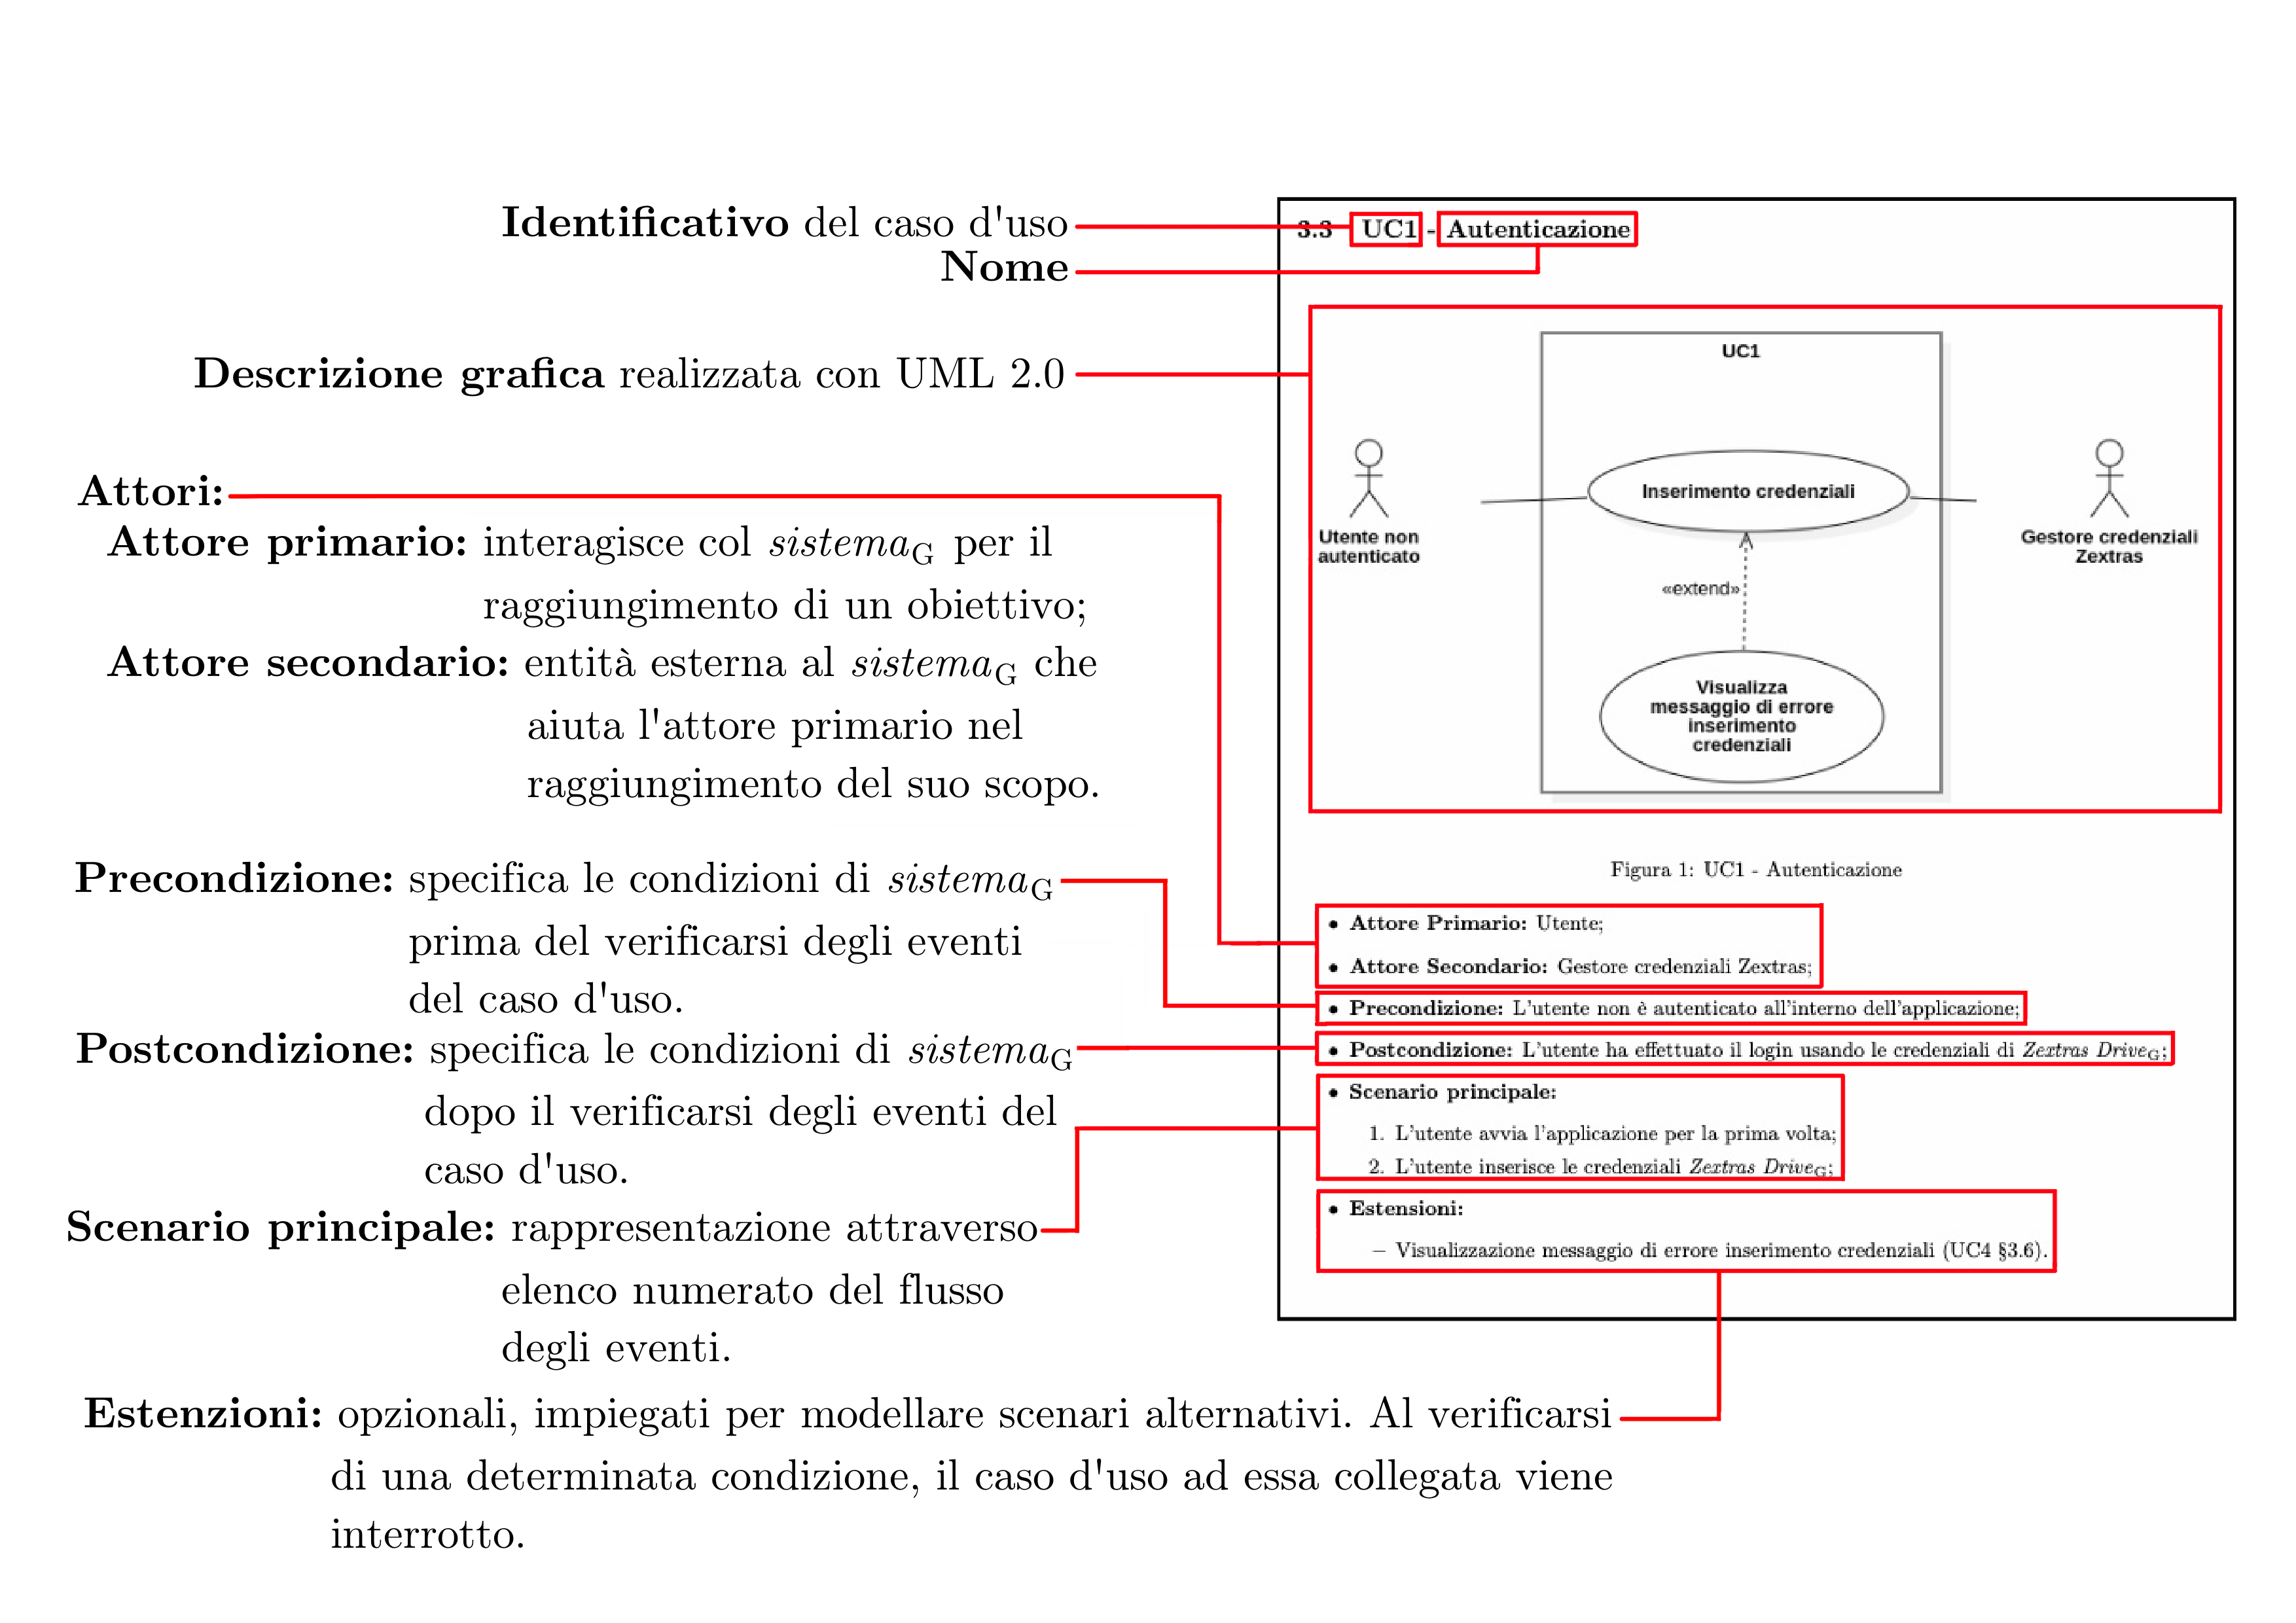
\includegraphics[scale = 0.6]{components/immagini/casouso.png}
    \caption{Struttura casi d'uso}
\end{figure}


\paragraph*{Qualità dei requisiti} 

\setlength{\freewidth}{\dimexpr\textwidth-0\tabcolsep}
	\renewcommand{\arraystretch}{1.5}
	\setlength{\aboverulesep}{0pt}
	\setlength{\belowrulesep}{0pt}
	\rowcolors{2}{AzzurroGruppo!10}{white}
	\begin{longtable}{L{.15\freewidth} L{.6\freewidth} L{.080\freewidth}}
		\rowcolor{AzzurroGruppo!30}
		\textbf{Qualità} & \textbf{Descrizione} \\
		\toprule
		\endhead		
		\textbf{Completezza} &  Descrizione specifica e dettagliata di ogni funzionalità richiesta dal prodotto \glo{software} e del suo comportamento in risposta agli input dati.\\
		\textbf{Consistenza} &  Non devono crearsi situazioni di contraddizione tra \glo{requisiti}.\\
		\textbf{Correttezza} &  Il requisito deve risultare veramente necessario e richiesto dagli utenti finali.\\
		\textbf{Univocità} & Ogni requisito deve essere contraddistinto da un codice formale univoco. \\
		\textbf{Modificabilità} &  Il requisito deve poter cambiare nel tempo in modo facile, completo, consistente e in modo da mantenere la struttura e lo stile.\\
		\textbf{Non ambiguità} &  Il requisito deve avere una sola interpretazione.\\
		\textbf{Priorità} &  Il requisito ha un identificatore che ne esprime l'importanza.\\
		\textbf{Verificabilità} &  Si deve poter verificare che l'applicazione realizzi il requisito individuato.\\
		\textbf{Tracciabilità} &  Il requisito ha un'origine chiara, un nome e un numero in modo da poterlo referenziare in futuro.\\
		\bottomrule
		\hiderowcolors
		\caption{Elementi che contribuiscono alla qualità dei requisiti}
	\end{longtable}

\subsubsection{Progettazione}

L'attività di progettazione definisce le caratteristiche che il prodotto richiesto deve avere in modo da fornire una soluzione che soddisfa i \glo{requisiti} specificati nell'\AdR{}. Oltre a garantire la qualità del prodotto applicando un approccio sistematico ai problemi, i compiti vengono suddivisi in modo da ridurre la complessità del problema iniziale e rendere più semplice la codifica da parte dei \progrs{}. Il compito di questi ultimi, in particolare, è quello di definire l'architettura logica del \glo{sistema}, che si adatta a ogni modifica effettuata nell'\AdR{}. Inoltre, l'architettura definita deve:
\begin{itemize}
\item essere comprensibile, modulare e robusta;
\item risultare affidabile, quindi svolgere i propri compiti ogni qual volta venga richiesto;
\item rispettare le caratteristiche di safety e security rispetto ai malfunzionamenti;
\item essere disponibile;
\item mostrare un utilizzo efficiente delle risorse necessarie;
\item garantire riusabilità;
\item presentare componenti semplici e coese nel raggiungimento degli obiettivi, incapsulate e con un basso livello di accoppiamento.
\end{itemize}
L'attività di progettazione può essere suddivisa in due parti:

\setlength{\freewidth}{\dimexpr\textwidth-0\tabcolsep}
	\renewcommand{\arraystretch}{1.5}
	\setlength{\aboverulesep}{0pt}
	\setlength{\belowrulesep}{0pt}
	\rowcolors{2}{AzzurroGruppo!10}{white}
	\begin{longtable}{L{.15\freewidth} L{.6\freewidth} L{.080\freewidth}}
		\rowcolor{AzzurroGruppo!30}
		\textbf{Nome} & \textbf{Descrizione} \\
		\toprule
		\endhead		
		\textbf{Technology Baseline} &  Descrive le specifiche della progettazione ad alto livello del prodotto e delle sue componenti, l'elenco dei diagrammi UML che saranno utilizzati per la realizzazione dell'architettura e i \glo{test} di \ignore{verifica}.\\
		\textbf{Product Baseline} & Rende ancora più dettagliata l'attività di progettazione, integrando ciò che è riportato nella Technology Baseline. Inoltre, definisce i \glo{test} necessari alla \glo{verifica}. \\
		\bottomrule
		\hiderowcolors
		\caption{Descrizione fasi di progettazione}
	\end{longtable}

\paragraph*{Design patterns}
Devono essere descritti i design pattern utilizzati per realizzare l'architettura. Ogni design pattern deve essere accompagnato da una descrizione e da un diagramma, che ne esponga il significato e la struttura.
\newpage
\paragraph*{Diagrammi UML 2.0}

{
\setlength{\freewidth}{\dimexpr\textwidth-0\tabcolsep}
	\renewcommand{\arraystretch}{1.5}
	\setlength{\aboverulesep}{0pt}
	\setlength{\belowrulesep}{0pt}
	\rowcolors{2}{AzzurroGruppo!10}{white}
	\begin{longtable}{L{.210\freewidth} L{.6\freewidth} L{.080\freewidth}}
		\rowcolor{AzzurroGruppo!30}
		\textbf{Tipo} & \textbf{Descrizione} \\
		\toprule
		\endhead		
		\textbf{Diagrammi delle attività} & Mostrano tutte le operazioni di una certa attività, anche fuori dal contesto. \\
		\textbf{Diagrammi delle classi} & Mostrano gli attributi e i metodi di classi e tipi.\\
		\textbf{Diagrammi dei package} & Mostrano i raggruppamenti tra le classi. \\
		\textbf{Diagrammi di sequenza} & Mostrano sequenze di azioni usando scelte definite.\\
		\bottomrule
		\hiderowcolors
		\caption{Descrizione dei diagrammi UML 2.0}
	\end{longtable}
}
\paragraph*{Test}
Ogni \prog{} avrà il compito di definire \glo{test} opportuni, che dovranno essere accompagnati da eventuali classi utili ad individuare errori ed anomalie.


\subsubsection{Codifica}
La codifica ha lo scopo di normare l'effettiva realizzazione del prodotto \glo{software} richiesto. Tramite questa attività si concretizza l'architettura di alto livello pensata dai \progs{} nel documento \PdQ{}. I \progrs{} dovranno attenersi a queste norme durante la fase di programmazione e implementazione. L'uso di norme e convenzioni è fondamentale per permettere la generazione di codice leggibile e uniforme, agevolare la manutenzione e i processi di \glo{verifica} e \glo{validazione}.
\paragraph*{Convenzioni per i nomi}
\
{
	\setlength{\freewidth}{\dimexpr\textwidth-0\tabcolsep}
	\renewcommand{\arraystretch}{1.5}
	\setlength{\aboverulesep}{0pt}
	\setlength{\belowrulesep}{0pt}
	\rowcolors{2}{AzzurroGruppo!10}{white}
	\begin{longtable}{L{.210\freewidth} L{.6\freewidth} L{.080\freewidth}} 
		\rowcolor{AzzurroGruppo!30}
		\textbf{Convenzione} & \textbf{Uso} \\
		\toprule
		\endhead		
		\textbf{\glo{PascalCase}} & Dichiarazione dei nomi delle classi. \\ 
		\textbf{\glo{Snake case}} & Dichiarazione dei nomi dei metodi e delle variabili.  \\
		\textbf{\_snake\_case} & Aggiunta di singolo underscore prima delle variabili o metodi privati.\\
		\textbf{Univocità nomi} & Nello scope della dichiarazione il nome usato esso deve essere univoco. \\
		\bottomrule
		\hiderowcolors
		\caption{Descrizione delle convenzioni nei nomi usati in codifica}
	\end{longtable}
}
\paragraph*{Convenzioni sulle pratiche}
\
{
	\setlength{\freewidth}{\dimexpr\textwidth-0\tabcolsep}
	\renewcommand{\arraystretch}{1.5}
	\setlength{\aboverulesep}{0pt}
	\setlength{\belowrulesep}{0pt}
	\rowcolors{2}{AzzurroGruppo!10}{white}
	\begin{longtable}{L{.210\freewidth} L{.6\freewidth} L{.080\freewidth}}
		\rowcolor{AzzurroGruppo!30}
		\textbf{Pratica} & \textbf{Descrizione norma} \\
		\toprule
		\endhead		
		\textbf{Indentazione} & Il codice dovrà essere indentato usando 4 spazi. \\ 
		\textbf{Spaziature} & Dovrà essere presente una spaziatura prima e dopo gli operatori binari e dopo le virgole. \\
		\textbf{Commenti} & Ogni commento deve essere separato con uno spazio dalla sua definizione e due spazi dal codice se si tratta di un commento inline. \\ 
		\textbf{Lunghezza della riga di codice} & Ogni riga di codice non deve superare 100 caratteri di lunghezza. \\
		\textbf{Brevità dei metodi} & Ogni blocco di codice non dovrà superare le 50 istruzioni. Se tuttavia questo risulta indispensabile può essere permesso, per questo la norma è consigliata e non obbligatoria.\\ 	
		\textbf{Stringhe} & Ogni stringa deve essere definita con singoli apici. \\
		\textbf{Funzioni} & Bisogna evitare quando possibile l'utilizzo di funzioni ricorsive.\\ 	
		\textbf{Variabili} & Non definire variabili che non verranno utilizzate.\\ 	
		\textbf{Operatori} & Ogni operatore dovrà essere preceduto e seguito da uno spazio.\\ 	
		\textbf{Complessità ciclomatica} & L'annidamento di cicli sarà evitato il più possibile. In questo modo le funzioni non saranno troppo onerose da eseguire e soprattutto godranno di una maggiore leggibilità. \\  			
		\bottomrule
		\hiderowcolors
		\caption{Descrizione delle norme delle pratiche di codifica}
	\end{longtable}
}

\subsubsection{Strumenti}
{
	\setlength{\freewidth}{\dimexpr\textwidth-0\tabcolsep}
	\renewcommand{\arraystretch}{1}
	\setlength{\aboverulesep}{0pt}
	\setlength{\belowrulesep}{0pt}
	\rowcolors{2}{AzzurroGruppo!10}{white}
	\begin{longtable}{L{.210\freewidth} L{.6\freewidth} L{.080\freewidth}}
		\rowcolor{AzzurroGruppo!30}
		\textbf{Nome} & \textbf{Descrizione} \\
		\toprule
		\endhead		
		\textbf{StarUML} & Strumento utilizzato per la creazione di diagrammi UML. Offre molte agevolazioni che permettono una produzione veloce dei diagrammi e risulta uno strumento di semplice apprendimento e uso.\\ 
		\textbf{PyCharm} & IDE pensato per lo sviluppo di codice con il linguaggio Python. \\
		\textbf{Visual Studio Code} & IDE molto popolare utilizzato per lo sviluppo in molteplici linguaggi di programmazione. \\		
		\bottomrule
		\hiderowcolors
		\caption{Strumenti utilizzati nel processo di sviluppo}
	\end{longtable}
	
	
\subsubsection{Metriche}

\subsubsection*{Metriche Codifica}

	\setlength{\freewidth}{\dimexpr\textwidth-0\tabcolsep}
	\renewcommand{\arraystretch}{1.5}
	\setlength{\aboverulesep}{0pt}
	\setlength{\belowrulesep}{0pt}
	\rowcolors{2}{AzzurroGruppo!10}{white}
	\begin{longtable}{L{.10\freewidth} L{.5\freewidth} L{.250\freewidth}}
		\rowcolor{AzzurroGruppo!30}
		\textbf{Codice} & \textbf{Descrizione} & \textbf{Formula}\\
		\toprule
		\endhead		
		\textbf{MCD01} & Rappresenta la percentuale degli errori gestiti nel codice. Un valore elevato indica la solidità del codice. & -\\
		\textbf{MCD02} & Usata per valutare la complessità dell'algoritmo, è basata sulla struttura del grafo che lo rappresenta. & \small{C=$(n^\circ\ archi)-(n^\circ\ nodi)+(2*n^\circ\ componentiDisconnesse)$} \\
		\textbf{MCD03} & Il codice non deve avere variabili inutilizzate, esse andrebbero ad intaccare le performance e la facilità di manutenzione del codice. & -\\
		\textbf{MCD04} & Indice che riporta la facilità con cui l'utente riesce a comprendere cosa fa il codice, rappresentata mediante il numero di linee di commento nel codice. & \small{R=$\frac{n^\circ\ linee\ commento}{n^\circ\ linee\ codice}$}  \\
		\textbf{MCD05} &  Metrica che riporta la quantità di codice coperta da \glo{test}. Più questo valore aumenta e più il codice può ricevere implementazioni ed il cliente utilizzarlo senza incorrere in problemi. & - \\
		\textbf{MCD06} & Per facilitare la lettura e la riduzione della complessità di una singola riga di codice non sarà possibile avere righe di codice più lunghe di quanto stabilito dalla metrica. & -\\
		\textbf{MCD07} & I metodi devono generalmente essere brevi per poter assicurare che la loro complessità non risulti eccessiva. & - \\
		\textbf{MCD08}& Misura il numero di classi che sono accoppiate a una particolare classe. Un accoppiamento eccessivo rende il sistema più difficile da gestire e riutilizzare. & - \\
		\textbf{MCD09} & Un elevato numero di parametri presenti all'interno dello stesso metodo indica il bisogno di ridurre le funzionalità associate a tale metodo. Più è elevato questo valore e più aumenta la possibilità di commettere errori progettuali. & - \\
		\textbf{MCD10} & Indica il livello di annidamento di un metodo. Un valore alto porta a un codice di difficile manutenzione, aumentandone la complessità.& - \\
		\bottomrule
		\hiderowcolors
		\caption{Descrizione metriche per il processo di codifica}\\
	\end{longtable}
	
\newpage{}
\subsubsection*{Metriche Progettazione}

	\setlength{\freewidth}{\dimexpr\textwidth-0\tabcolsep}
	\renewcommand{\arraystretch}{1}
	\setlength{\aboverulesep}{0pt}
	\setlength{\belowrulesep}{0pt}
	\rowcolors{2}{AzzurroGruppo!10}{white}
	\begin{longtable}{L{.10\freewidth} L{.5\freewidth} L{.350\freewidth}}
		\rowcolor{AzzurroGruppo!30}
		\textbf{Codice} & \textbf{Descrizione} & \textbf{Formula}\\
		\toprule
		\endhead		
		
		\textbf{MPR01} & Indica se si è in linea, in anticipo oppure in ritardo rispetto alla pianificazione delle attività di progetto. & \small{P01=$P07-P06$}\\
		\textbf{MPR02} & Indica se alla data corrente si è speso di più o di meno rispetto al budget totale pianificato. & \small{P02=$P06-P05$}\\
		\textbf{MPR03} & Indica la percentuale dei \glo{requisiti} obbligatori soddisfatti. & \small{P03=$\frac{n^\circ\ r. obbligatori\ soddisfatti*100}{n^\circ\ totale\ r. obbligatori}$}\\
		\textbf{MPR04} & Indica la percentuale dei \glo{requisiti} opzionali soddisfatti. & \small{P04=$\frac{n^\circ\ r. opzionali\ soddisfatti*100}{n^\circ\ totale\ r. opzionali}$}\\
		\textbf{MPR05} & Indica il denaro speso fino al momento del calcolo. & \small{P05=$\sum (ore\ lavorative*corrispondente\ costo\ orario)$}\\ 
		\textbf{MPR06} & Rappresenta il costo pianificato per realizzare le attività di progetto fino al momento del calcolo. & \small{P06=$\% lavoro\ pianificato*tot. budget$}\\
		
		\bottomrule
		\hiderowcolors
		\caption{Descrizione metriche per il processo di progettazione}\\
	\end{longtable}
